%% LyX 2.1.1 created this file.  For more info, see http://www.lyx.org/.
%% Do not edit unless you really know what you are doing.
\documentclass[twocolumn,pre, reprint, nofootinbib]{revtex4-1}
\usepackage[latin9]{inputenc}
\setcounter{secnumdepth}{3}
\usepackage{amssymb}
\usepackage{graphicx}
\usepackage{amsmath}


\newcommand\blfootnote[1]{%
  \begingroup
  \renewcommand\thefootnote{}\footnote{#1}%
  \addtocounter{footnote}{-1}%
  \endgroup
}
\makeatletter

%%%%%%%%%%%%%%%%%%%%%%%%%%%%%% LyX specific LaTeX commands.
%% Because html converters don't know tabularnewline
\providecommand{\tabularnewline}{\\}

%%%%%%%%%%%%%%%%%%%%%%%%%%%%%% Textclass specific LaTeX commands.
% Fix a couple of bugs in REVTeX 4.1
\def\lovname{List of Videos}
\@ifundefined{textcolor}{}
{
 \definecolor{BLACK}{gray}{0}
 \definecolor{WHITE}{gray}{1}
 \definecolor{RED}{rgb}{1,0,0}
 \definecolor{GREEN}{rgb}{0,1,0}
 \definecolor{BLUE}{rgb}{0,0,1}
 \definecolor{CYAN}{cmyk}{1,0,0,0}
 \definecolor{MAGENTA}{cmyk}{0,1,0,0}
 \definecolor{YELLOW}{cmyk}{0,0,1,0}
}

\makeatother

\begin{document}

\title{Anti-ferromagnetic Ising Model in Hierarchical Networks }


\author{Xiang Cheng and Stefan Boettcher}

\affiliation{Department of Physics, Emory University, Atlanta, GA 30322, USA}
\begin{abstract}
The Ising antiferromagnet  is a convenient model of glassy dynamics.  It can introduce geometric frustrations and may give rise to a spin glass phase and glassy relaxation at low temperatures.  We apply the antiferromagnetic Ising model to 3 hierarchical networks which share features of both small world networks and regular lattices. Their recursive and fixed structures make them suitable for exact renormalization group analysis as well as numerical simulations. We first explore the dynamical behaviors using simulated annealing and discover an extremely slow relaxation at low temperatures. Then we employ the Wang-Landau algorithm to investigate the energy landscape and the corresponding equilibrium behaviors for different system sizes. Besides the Monte Carlo methods, renormalization group is used to study the equilibrium properties in the thermodynamic limit and to compare with the results from simulated annealing and Wang-Landau sampling. 
\smallskip 
\end{abstract}

\maketitle

\section{Introduction}

\label{sec:intro} 
The Ising antiferromagnet can introduce geometric frustrations and may give rise to interesting dynamics and phases. What may make it more interesting is that we are applying the antiferromagnetic model to hierarchical networks which have a lattice backbone and small-world structure. These networks could produce different critical phenomena from that found on lattice geometries (cite BoettcherEPL15 1-4).

\section{RG Calculations}
\label{sec:RG}
 The setup of renormalization is started by separating the Ising Hamiltonian into hierarchies
\begin{equation}
-\beta\mathcal{H} = \sum_{n=1}^{k-2} (-\beta \mathcal{H}_n)+ \mathcal{R}(K_2, K_3, \cdots)
\end{equation}
where $\mathcal{R}$ is the coupling beyond $\mathcal{H}_n$ of levels $k>2$. $\mathcal{H}_n$ depends on the interactions $K_0$ on the backbone and $L_0$, $L_1$, $K_1, \cdots$ among the long range couplings. We describe the RG procedure network by network. 

\subsection{Ising ferromagnet on HN3 and HN5}
\label{sec:hn35rgfm}
The Hamiltonian with magnetic field is
\begin{eqnarray}
\label{eq:hpz0}
 -\beta \mathcal{H}_n &=& K_0 \left(x_{n-2}x_{n-1} + x_{n-1}x_{n} +  x_{n}x_{n+1} +  x_{n+1}x_{n+2}\right) \nonumber \\ 
   && + K_1(x_{n-1}x_{n+1}) + yL_1(x_{n-2} x_{n+2}) \nonumber \\
   && +L_0(x_{n-2}x_{n} + x_{n}x_{n+2})  + 4I \nonumber\\
   && +\frac{H_K}{2}(x_{n-2} + 2x_{n-1}+2x_n+2x_{n+1}+x_{n+2})\nonumber\\
   && +\frac{H_L}{2}(x_{n-2}+2x_n + x_{n+2}) + \frac{H}{2}(x_{n-1}+x_{n+1})\nonumber\\
   && + \frac{T}{2}(x_{n-2}x_{n-1}x_n + x_n x_{n+1} x_{n+2})
\end{eqnarray}
where $y=0$ for HN3 and $y=1$ for HN5.

\subsubsection{ Magnetization}
The first is the plot of the magnetization vs temperature at small H which can just break the $Z2$ symmetry.  
\begin{figure}[h]
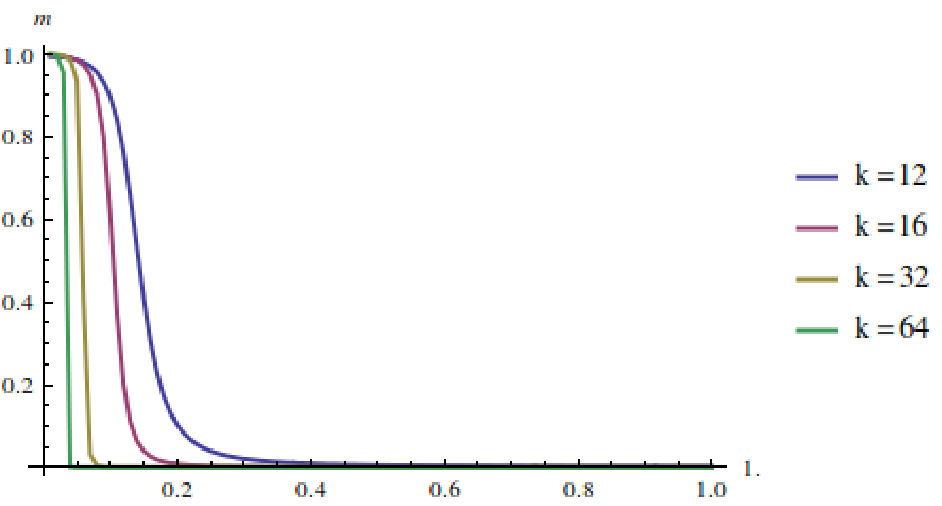
\includegraphics[width=1\columnwidth]{../Maca/figures/HN3_FM_m.pdf}
\caption{HN3 Ising Ferromagnet magnetization vs temperature $\mu$. This figure shows that the transition temperature is 0. }
\end{figure}

\begin{figure}[h]
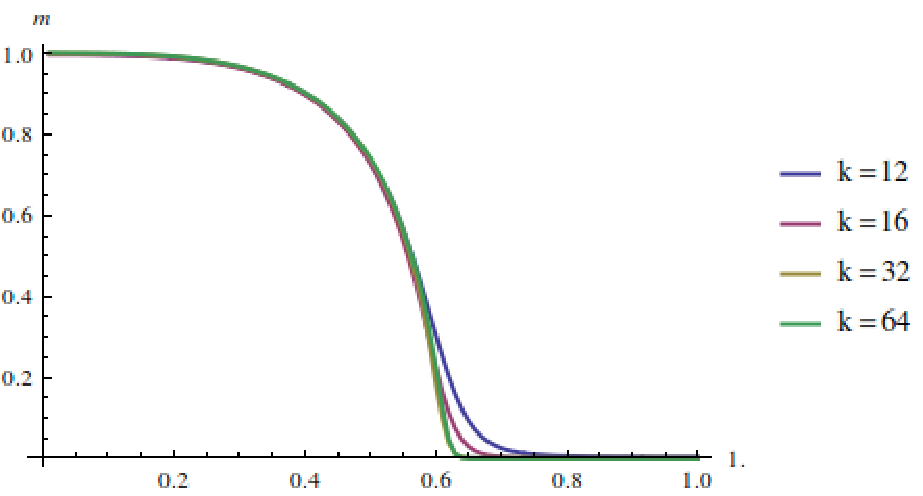
\includegraphics[width=1\columnwidth]{../Maca/figures/HN5_FM_m.pdf}
\caption{HN5 Ising Ferromagnet magnetization vs temperature $\mu$. This figure shows that the transition temperature is around 0.62 which should be same as the $\mu_c = 0.618033...$ found by fixed point analysis in BoettcherPRE01\cite{boettcher2011rg}. \\
This figure could look better if I finely tune the magnetic filed.
}
\end{figure}

I also try to make a plot similar to Nowaga's Fig 3 \cite{nogawa12} 
In our case, $t =\  2e^{-K_0}-1 \ = \ 2\sqrt{\mu}-1 $. Thus, the $x-$axis is $|t|\ln H^{-1}$, and the $y-$axis is $m \sqrt{\ln H^{-1}}$. The figures for HN3 and HN5 for $N=2^{16}$ are shown in Fig. \ref{fig:hn3fmmt} and Fig. \ref{fig:hn5fmmt}.

As you can see, the pattern and magnitude of $y$ is very different from Nowaga's results. Part of reason may be because they are using different network and different Hamiltonian ($\sum \delta_{\sigma_i,\sigma_j} + \sum \delta_{\sigma_i,0}$). It seems that, for magnetization, there is no symmetry because of their setup  $\delta_{\sigma_i,0}$.
\begin{figure}[h]
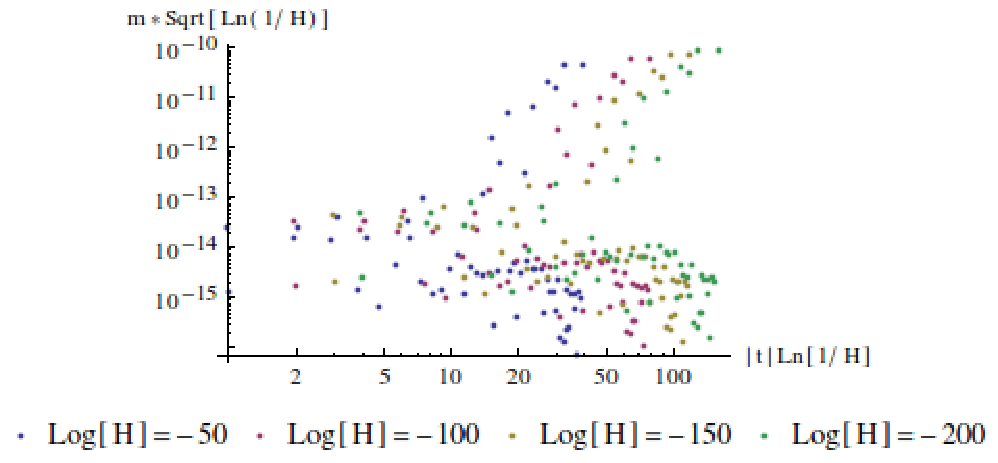
\includegraphics[width=1\columnwidth]{../Maca/figures/HN3_FM_m_t1.pdf}
\caption{HN3 Ising Ferromagnet $N=2^{16}$. }
\label{fig:hn3fmmt}
\end{figure}
\begin{figure}[h]
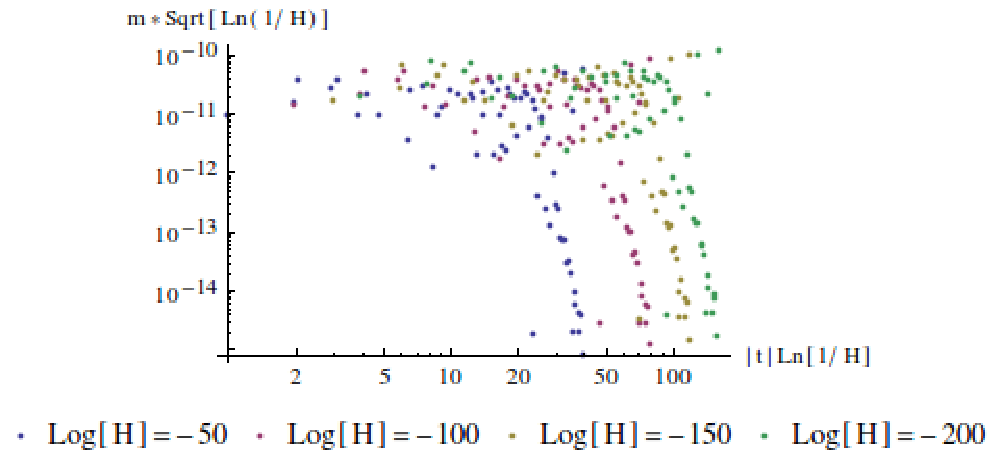
\includegraphics[width=1\columnwidth]{../Maca/figures/HN5_FM_m_t1.pdf}
\caption{HN5 Ising Ferromagnet $N=2^{16}$.  }
\label{fig:hn5fmmt}
\end{figure}

\subsubsection{Specific Heat and Susceptibility: HN5 FM}
Only HN5 results are shown here. 

\begin{figure}[h]
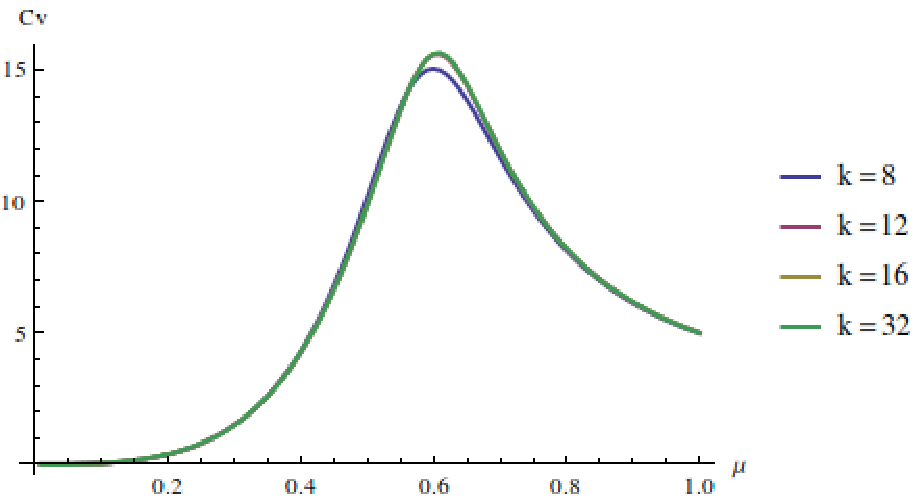
\includegraphics[width=1\columnwidth]{../Maca/figures/HN5_FM_Cv.pdf}
\caption{HN5 Ising Ferromagnet Specific Heat.  }
\label{fig:hn5fmcv}
\end{figure}

\begin{figure}[h]
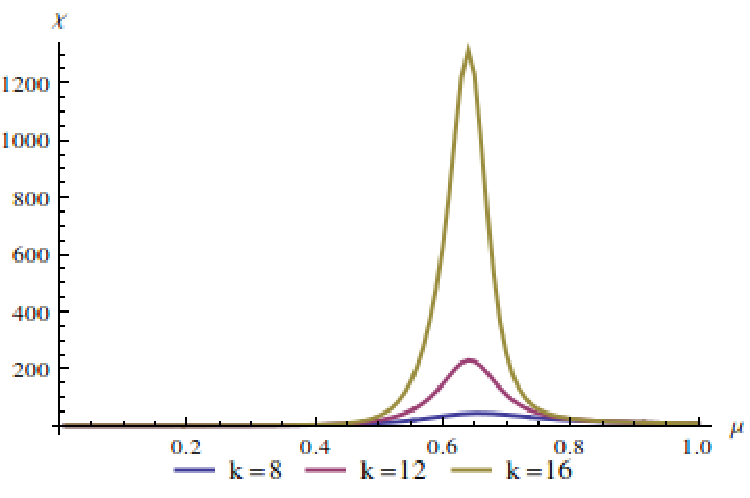
\includegraphics[width=1\columnwidth]{../Maca/figures/HN5_FM_x.pdf}
\caption{HN5 Ising Ferromagnet Susceptibility in linear scale. It would look better if I tune more the magnetic filed to break the Z2 symmetry. But it is slow to run.}
\label{fig:hn5fmx}
\end{figure}

\begin{figure}[h]
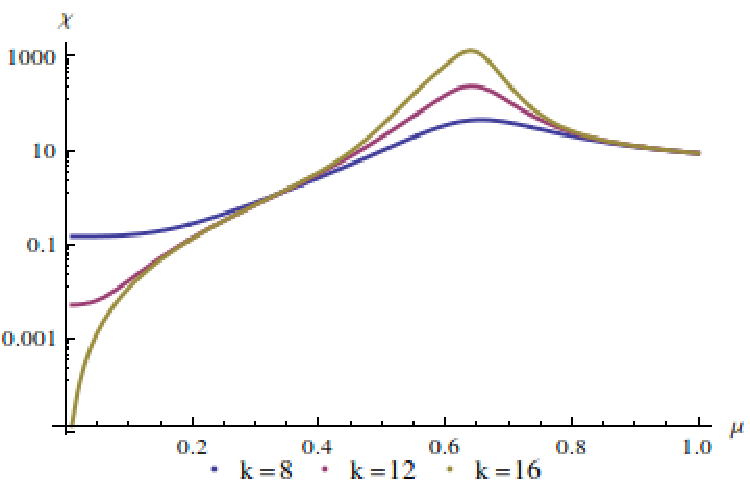
\includegraphics[width=1\columnwidth]{../Maca/figures/HN5_FM_x_log.pdf}
\caption{HN5 Ising Ferromagnet Susceptibility in log scale. It would look better if I tune more the magnetic filed to break the Z2 symmetry.  }
\label{fig:hn5fmx2}
\end{figure}


\subsection{Ising ferromagnet on HNNP}
\label{sec:hnnpfmrg}
The Hamiltonian with magnetic field is
\begin{eqnarray}
\label{eq:hpz0}
 -\beta \mathcal{H}_n &=& K_0 \left(x_{n-2}x_{n-1} + x_{n-1}x_{n} +  x_{n}x_{n+1} +  x_{n+1}x_{n+2}\right) \nonumber \\ 
   && + K_1(x_{n-2}x_{n+1} + x_{n-1}x_{n+2}) + yL_1(x_{n-2} x_{n+2}) \nonumber \\
   && +L_0(x_{n-2}x_{n} + x_{n}x_{n+2})  + 4I \nonumber\\
   && +\frac{H_K}{2}(x_{n-2} + 2x_{n-1}+2x_n+2x_{n+1}+x_{n+2})\nonumber\\
   && +\frac{H_L}{2}(x_{n-2}+2x_n + x_{n+2}) + \frac{H}{2}(x_{n-1}+x_{n+1})\nonumber\\
   && + \frac{T}{2}(x_{n-2}x_{n-1}x_n + x_n x_{n+1} x_{n+2})
\end{eqnarray}
where $y=0$ is for HNNP, and $y=1$ is for HN6. Here we discuss HNNP first, so $y=0$.
Based on fixed point analysis, $\mu_c = 0.553 814 426 157 623 . . .$. We now check the magnetization to see whether the transition temperature is the same or not.

\subsubsection{Magnetization : HNNP FM}

\begin{figure}[h]
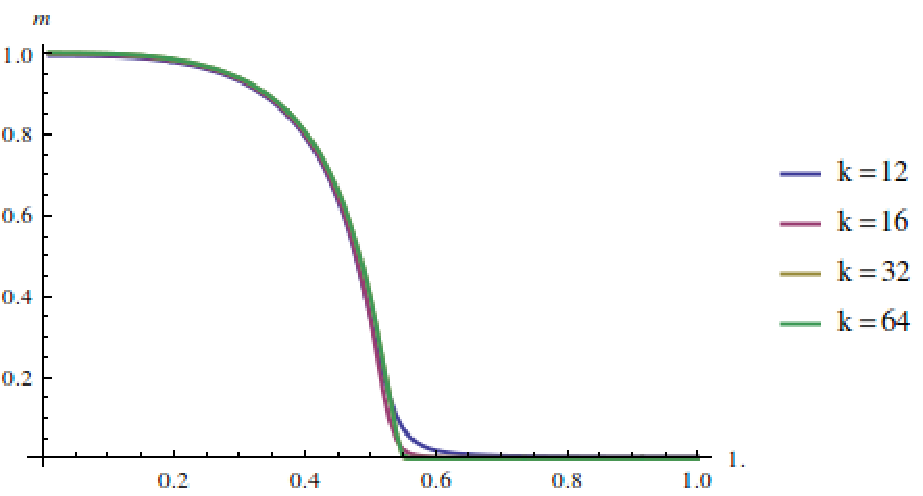
\includegraphics[width=1\columnwidth]{../Maca/figures/HNNP_FM_m.pdf}
\caption{HNNP Ising Ferromagnet magnetization vs temperature $\mu$. This figure shows that the transition temperature is around 0.55 which should be same as the $\mu_c = 0.5538...$ found by fixed point analysis in BoettcherPRE01\cite{boettcher2011rg}. \\
This figure could look better if I finely tune the magnetic filed.
}
\end{figure}

\begin{figure}[h]
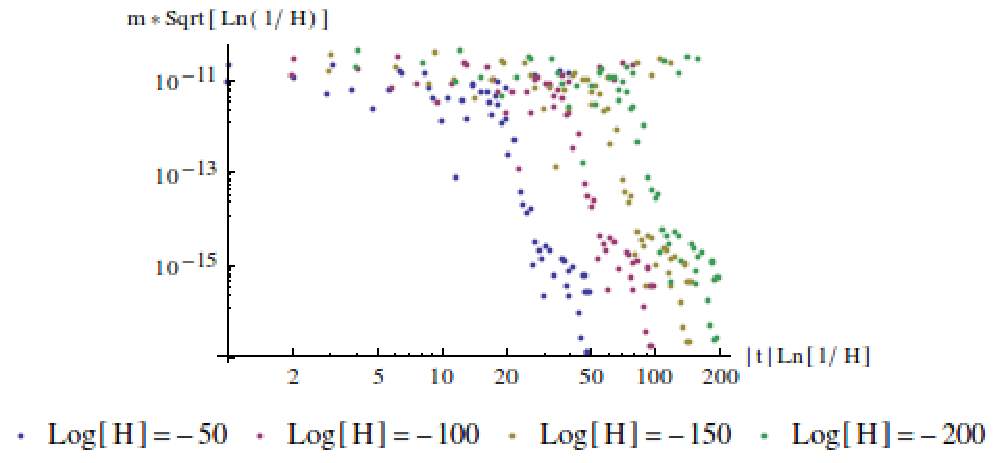
\includegraphics[width=1\columnwidth]{../Maca/figures/HNNP_FM_mt1.pdf}
\caption{HNNP Ising Ferromagnet $N=2^{16}$.  }
\label{fig:hnnpfmmt}
\end{figure}

\subsubsection{Specific Heat and Susceptibility : HNNP FM}
\begin{figure}[h]
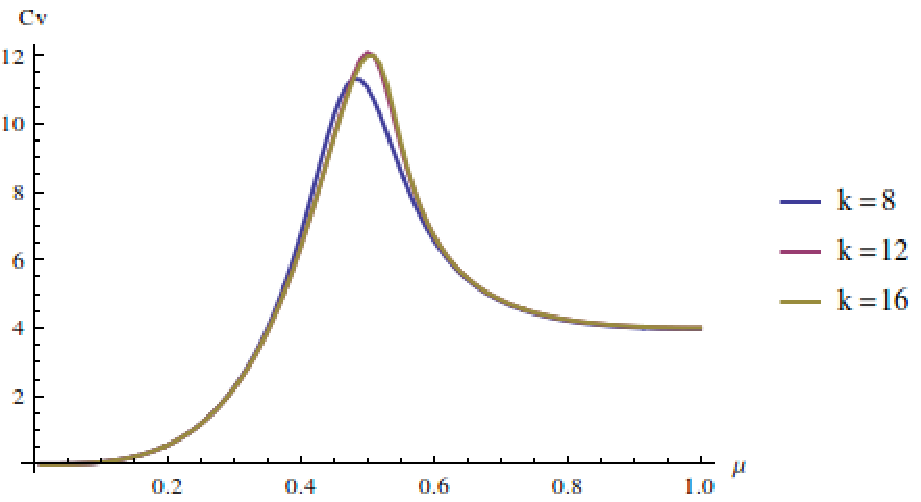
\includegraphics[width=1\columnwidth]{../Maca/figures/HNNP_FM_Cv.pdf}
\caption{HNNP Ising Ferromagnet Specific Heat.  }
\label{fig:hnnpfmcv}
\end{figure}

\begin{figure}[h]
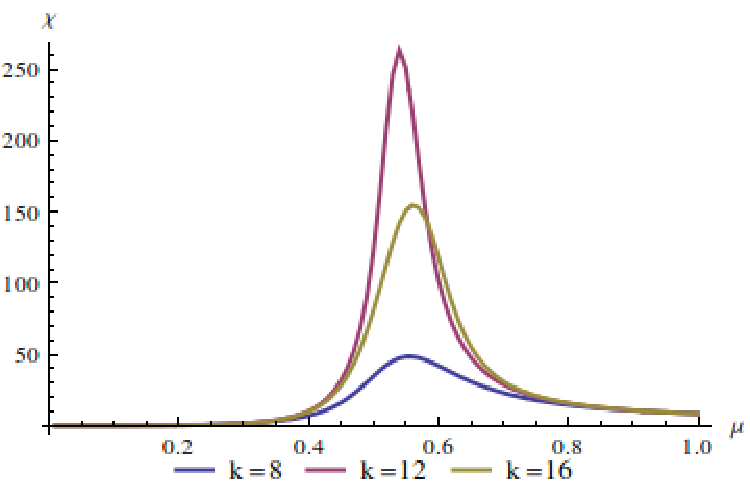
\includegraphics[width=1\columnwidth]{../Maca/figures/HNNP_FM_x.pdf}
\caption{HNNP Ising Ferromagnet Susceptibility in linear scale. It would look better if I tune more the magnetic filed to break the Z2 symmetry. But it is slow to run.}
\label{fig:hnnpfmx}
\end{figure}

\begin{figure}[h]
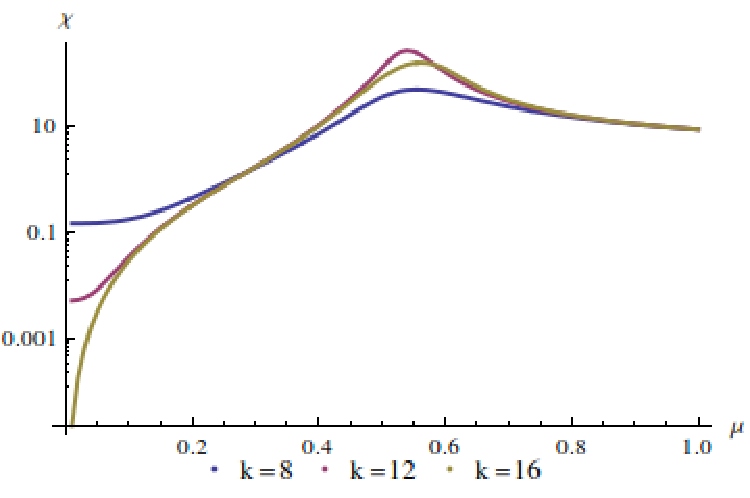
\includegraphics[width=1\columnwidth]{../Maca/figures/HNNP_FM_x_log.pdf}
\caption{HNNP Ising Ferromagnet Susceptibility in log scale. It would look better if I tune more the magnetic filed to break the Z2 symmetry.  }
\label{fig:hnnpfmx2}
\end{figure}



\subsection{Ising antiferromagnet on HN3 and HN5}
\label{sec:hn35rg}
working on it; 
preliminary results should be available next Tuesday.

\subsection{Ising antiferromagnet on HNNP}
\label{sec:hnnprg}
working on it; 
preliminary results should be available next Tuesday.

\bibliographystyle{apsrev4-1}
%\bibliography{Jamming}
\bibliography{cheng}

\end{document}
